\documentclass{article}
\usepackage{listings}
\usepackage{graphicx}
\usepackage{pythonhighlight}
\title{Week2 Report}
\author{Zhang Heartbright}
\date{\today}
\usepackage[a4paper]{geometry}

\begin{document}
\maketitle
\begin{abstract}
    This time, I put my effort on coding, setting environment of python, and spend efforts on using VS Code which treats me most friendly.\par
    To sum up what I have down this week, it can be concluded as below:\par
        1. Reset the operation system for 3 times, beacuse I have so messed up installing the extentions \par
        2. Learning to use VS Code to code everything, python, c++, markdown, and latex\par
        3. Find the homework of Deeplearning and code them.\par
    Summary: I hate this week \par
\end{abstract}
\tableofcontents
\newpage
\section{Homework First}
\subsection{Building basic functions with numpy}
Numpy is the main package for scientific computing in Python.
It is maintained by a large community (www.numpy.org).
In this exercise you will learn several key numpy functions such as np.exp, np.log, and np.reshape.
You will need to know how to use these functions for future assignments.\par
$sigmoid(x)$ = $\frac{1}{1+e^{-x}}$(also known as the logistic function)

\begin{python}
import numpy as np
#Exercise_1: Implement the sigmoid function using numpy.

def sigmod(x):
    s=1/(1+np.exp(x))
    return s

x=np.array([1,2,3])
print ("sigmod is "+str(sigmod(x)))
\end{python}
\newpage
\subsection{Sigmoid gradient}
Implement the function sigmoid\_grad to compute the gradient of the sigmoid function with respect to its input x. The formula is: \par
 sigmoid\_derivative(x) = $\sigma(x)$ = $\sigma'(x)$ (1 - $\sigma(x)$)
\begin{python}
    def sigmoid_derivative(x):
    s=sigmod(x)
    ds=s*(1-s)
    return ds
print("sigmoid_derivative is "+str(sigmoid_derivative(x)))
\end{python}
\newpage
\subsection{ Reshaping arrays}
Two common numpy functions used in deep learning are np.shape and np.reshape().\par
- X.shape is used to get the shape (dimension) of a matrix/vector X.\par
- X.reshape(��) is used to reshape X into some other dimension. \par
\begin{figure}[htbp]
    \centering
    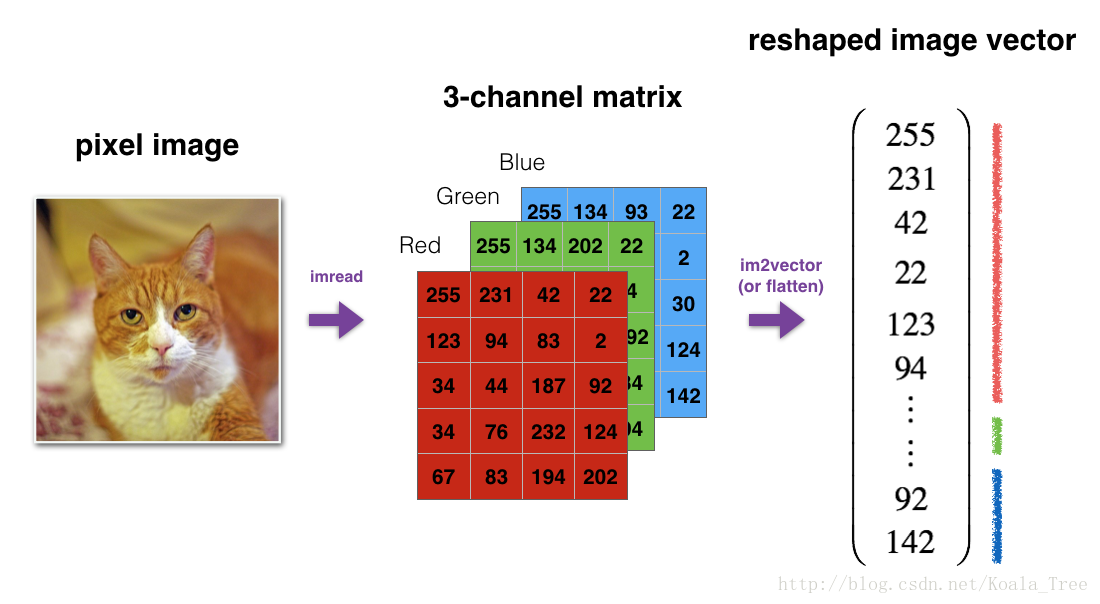
\includegraphics[width=10cm]{pixel_image.png}
\end{figure}[htbp]
\begin{python}
    def image2vector(image):
    res = image.reshape((image.shape[0] * image.shape[1] * image.shape[2], 1))
    return res
image = np.array([[[ 0.67826139,  0.29380381],
        [ 0.90714982,  0.52835647],
        [ 0.4215251 ,  0.45017551]],

       [[ 0.92814219,  0.96677647],
        [ 0.85304703,  0.52351845],
        [ 0.19981397,  0.27417313]],

       [[ 0.60659855,  0.00533165],
        [ 0.10820313,  0.49978937],
        [ 0.34144279,  0.94630077]]])
print("image reshaped like this "+"\n"+str(image2vector(image)))
###### And result returns:
"""
image2vector(image) = [[ 0.67826139]
 [ 0.29380381]
 [ 0.90714982]
 [ 0.52835647]
 [ 0.4215251 ]
 [ 0.45017551]
 [ 0.92814219]
 [ 0.96677647]
 [ 0.85304703]
 [ 0.52351845]
 [ 0.19981397]
 [ 0.27417313]
 [ 0.60659855]
 [ 0.00533165]
 [ 0.10820313]
 [ 0.49978937]
 [ 0.34144279]
 [ 0.94630077]]
 """
\end{python}
\newpage
\subsection{Broadcasting}
A very important concept to understand in numpy is ��broadcasting��.
It is very useful for performing mathematical operations between arrays of different shapes.
For the full details on broadcasting, you can read the official broadcasting documentation.\par
\begin{python}
    def broadcast(x,y):
    s=x/y
    return s


X=np.array([[1,2,3],
            [4,5,6]])
X_2=np.array([[5.0],
             [2.0]])
print(broadcast(X,X_2))
#### And Result is :
"""
[[0.2 0.4 0.6]
 [2.  2.5 3. ]]
"""
\end{python}
\newpage
\subsection{Implement the L1 and L2 loss functions}
Implement the numpy vectorized version of the L1 loss. You may find the function abs(x) (absolute value of x) useful.
\begin{python}
import numpy as np
def L1(yhat, y):
    loss = np.sum(np.abs(y - yhat))
    return loss
yhat = np.array([.9, 0.2, 0.1, .4, .9])
y = np.array([1, 0, 0, 1, 1])
print("L1 = " + str(L1(yhat,y)))
#########---L1---#########
def L2(yhat, y):
    loss =np.sum(np.power((y - yhat), 2))
    return loss
yhat = np.array([.9, 0.2, 0.1, .4, .9])
y = np.array([1, 0, 0, 1, 1])
print("L2 = " + str(L2(yhat,y)))
\end{python}
\newpage
\section{Logistic Regression with a Neural Network mindset }
\begin{abstract}
- numpy is the fundamental package for scientific computing with Python.\par
- h5py is a common package to interact with a dataset that is stored on an H5 file.\par
- matplotlib is a famous library to plot graphs in Python.\par
- PIL and scipy are used here to test your model with your own picture at the end.\par
\end{abstract}
\begin{python}
    ### Fllows are packages
import numpy as np
import matplotlib.pyplot as plt
import h5py
import scipy
from PIL import Image
from scipy import ndimage
from lr_utils import load_dataset

### Load Data
### load_dataset �����Ѿ���ǰ��һ�Ѹ�ֵ����
train_set_x_orig, train_set_y, test_set_x_orig, test_set_y, classes = load_dataset()
index = 25
plt.imshow(train_set_x_orig[index])
print ("y = " + str(train_set_y[:, index]) + ", it's a '" + classes[np.squeeze(train_set_y[:, index])].decode("utf-8") +  "' picture.")
\end{python}
\begin{python}
    #####Fllows  are lr_utils.py
import numpy as np
import h5py


def load_dataset():
    train_dataset = h5py.File('datasets/train_catvnoncat.h5', "r")
    train_set_x_orig = np.array(train_dataset["train_set_x"][:]) # your train set features
    train_set_y_orig = np.array(train_dataset["train_set_y"][:]) # your train set labels

    test_dataset = h5py.File('datasets/test_catvnoncat.h5', "r")
    test_set_x_orig = np.array(test_dataset["test_set_x"][:]) # your test set features
    test_set_y_orig = np.array(test_dataset["test_set_y"][:]) # your test set labels

    classes = np.array(test_dataset["list_classes"][:]) # the list of classes

    train_set_y_orig = train_set_y_orig.reshape((1, train_set_y_orig.shape[0]))
    test_set_y_orig = test_set_y_orig.reshape((1, test_set_y_orig.shape[0]))

    return train_set_x_orig, train_set_y_orig, test_set_x_orig, test_set_y_orig, classes
\end{python}
\newpage
\section{Summary}
 The vedios are easy to get through, and the new concepts to be understand are not that difficult, but to program it is really challenging.\par
 However, the most challenging part is to build the proper environment, and make sure your OS is in healthy condition.
\end{document}
